\documentclass[11pt]{article}

\usepackage[review]{acl}

\usepackage{times}
\usepackage{latexsym}
\usepackage[T1]{fontenc}
\usepackage[utf8]{inputenc}
\usepackage{microtype}
\usepackage{graphicx}
\usepackage{booktabs}
\usepackage{amsmath}
\usepackage{amssymb}
\usepackage{xcolor}

\newcommand{\placeholder}[1]{\textcolor{red}{[#1]}}

\title{The Embedding Alignment Gap: Why Diversity-Based Data Selection\\Accelerates Model Collapse in Iterative Self-Training}

\author{Anonymous}

\begin{document}
\maketitle

\begin{abstract}
Iterative self-training on model-generated data risks \emph{model collapse}---a progressive degradation of output quality across generations. A natural mitigation is diversity-based data curation: selecting training subsets that maximize coverage in the model's own embedding space. We show that this intuitive strategy backfires. In controlled iterative self-training experiments with GPT2 (125M and 355M parameters) on WikiText-103, Representation-Guided Diversity Selection (RGDS)---which uses the training model's embeddings to greedily maximize diversity---\emph{accelerates} collapse rather than preventing it, producing over 70\% higher perplexity than a random selection baseline operating under the same 50\% data budget ($74.29 \pm 7.71$ vs.\ $43.18 \pm 1.43$, $n{=}3$). We identify the mechanism behind this failure as the \emph{Embedding Alignment Gap}: the model's internal notion of ``diversity'' progressively diverges from actual content diversity as its representations co-degrade with the generated data, causing the mean selection ratio to decline from approximately 1.0 to $0.64 \pm 0.20$ over eight generations. Critically, all selection strategies that bypass the model's own embeddings---random sampling (PPL 43.18$\pm$1.43), external frozen embeddings (PPL 46.36$\pm$2.97), and uncurated full-corpus training (PPL 47.04$\pm$2.90)---cluster within a narrow perplexity range with no catastrophic failure. Meanwhile, standard representation quality diagnostics such as RankMe effective dimensionality and $k$-NN accuracy remain stable throughout training, rendering the alignment gap invisible to conventional monitoring. Our results demonstrate that coupling data selection to co-degrading internal representations creates a feedback loop that amplifies rather than mitigates collapse, and that zero-cost random sampling is a more robust alternative for iterative self-training pipelines.
\end{abstract}

\section{Introduction}

Training language models on their own generated data across multiple iterations leads to \emph{model collapse}---a progressive degradation in both output quality and lexical diversity \citep{shumailov2024ai, alemohammad2024self}. Each generation of synthetic data carries distributional artifacts from its parent model; when these artifacts compound across iterations, the distribution's tails erode and the model converges toward a narrow, repetitive mode \citep{seddik2024how, briesch2023large, guo2024curious}. As synthetic data becomes an increasingly prevalent component of training pipelines, understanding this feedback loop---and identifying strategies that avoid it---has become a pressing concern \citep{dohmatob2025strong, gerstgrasser2024model}.

Diversity-based data curation is a natural mitigation strategy. If model collapse arises from training on redundant or low-quality synthetic samples, then selecting a maximally diverse subset should preserve the distributional richness that iterative training erodes. Submodular maximization over embedding spaces provides a principled framework for this goal: submodular diversity objectives identify representative subsets that maximize geometric coverage of the data distribution \citep{wei2015submodularity, mirzasoleiman2020coresets}. Embedding-based selection has demonstrated strong results in data pruning \citep{sorscher2022beyond} and data-efficient training more broadly \citep{xie2023data, xia2024less, engstrom2024dsdm}. When the model's own representations define the embedding space, diversity selection should---in principle---directly counteract the homogenization that drives collapse.

We test this intuition in a controlled iterative self-training experiment and find the opposite. Representation-Guided Diversity Selection (RGDS)---which selects the most diverse 50\% of synthetic data according to the training model's own last-hidden-layer embeddings---increases Generation~7 perplexity by +72\% relative to random selection under the same data budget ($74.29 \pm 7.71$ vs.\ $43.18 \pm 1.43$, $n{=}3$) and reduces rare n-gram survival by 38\%. The method designed to preserve diversity accelerates collapse instead.

Existing data selection methods---SemDeDup \citep{abbas2023semdedup}, D4 \citep{tirumala2023d4}, DSIR \citep{xie2023data}---are designed for one-shot curation of static datasets where the embedding model is fixed. Active learning accounts for model updates between selection rounds \citep{ash2020deep, kirsch2019batchbald}, but not for the compound effect of selection bias feeding back into the selecting model's own training data across generations. The concept drift literature establishes that representations degrade under distribution shift \citep{lu2019learning, gama2014survey}; however, the interaction between this degradation and embedding-based selection in a self-consuming training loop---where the selecting model is also shaped by its selections---has not been quantified.

We trace this failure to the \emph{embedding alignment gap}: a progressive divergence between what the model's internal representations treat as ``diverse'' and what constitutes genuine content diversity. We quantify this divergence with the \emph{selection ratio}---the mean rare n-gram density of the selected subset divided by that of the rejected subset. A ratio above~1 indicates that the selected samples are richer in rare n-grams than the rejected samples; below~1, the selection preferentially retains content-poor samples. For RGDS, the selection ratio declines from ${\sim}1.0$ at Generation~0 to $0.64 \pm 0.20$ at Generation~7 ($n{=}3$): by the final generation, the model's internal notion of diversity has inverted relative to content diversity.

The sharpest evidence for the embedding alignment gap comes from comparing methods that share identical selection algorithms but differ in their embedding source. All methods that bypass internal embeddings cluster in a narrow band at Generation~7: Random~50\% ($43.18 \pm 1.43$), External-only using frozen Contriever \citep{izacard2022unsupervised} embeddings ($46.36 \pm 2.97$), and Uncurated ($47.04 \pm 2.90$)---all $n{=}3$ (ANOVA $p = 0.219$). Only RGDS produces catastrophic outcomes ($74.29 \pm 7.71$). The External-only method is particularly informative: it applies the same diversity selection algorithm and 50\% budget as RGDS but uses a frozen encoder whose embeddings do not co-degrade with training. Its normal-range performance confirms that the selection algorithm itself is not at fault---the failure arises specifically from using co-degrading internal embeddings as the selection criterion, a form of Goodhart's law in representation space \citep{gao2023scaling, karwowski2024goodhart}.

Our contributions are:
\begin{enumerate}
    \item We quantify the \emph{embedding alignment gap} via the \emph{selection ratio} and show that it worsens progressively, declining from ${\sim}1.0$ to $0.64 \pm 0.20$ over 8 generations of internal-embedding selection ($n{=}3$).
    \item We isolate the failure to internal embeddings specifically: RGDS is the only method producing catastrophic degradation, while random selection, frozen external embeddings, and no selection all cluster in a narrow performance band (Generation~7 PPL 43--50, ANOVA $p = 0.219$, $n{=}3$).
    \item We establish that the alignment gap causes accelerated collapse: under the same 50\% data budget, RGDS increases perplexity by +72\% and reduces rare n-gram survival by 38\% relative to random selection ($n{=}3$), with preliminary evidence of the same pattern at 355M parameters.
\end{enumerate}

\section{Related Work}

\subsection{Model Collapse in Iterative Training}

\citet{shumailov2024ai} demonstrate that language models trained recursively on their own generated data undergo irreversible tail distribution erosion, establishing model collapse as a fundamental limitation of self-consuming training loops. \citet{dohmatob2024tale} further analyze this through scaling laws, showing that synthetic data truncates heavy-tailed input distributions, causing loss of scaling and skill degradation---directly relevant to the rare n-gram tail erosion we observe. \citet{alemohammad2024self} formalize this as Model Autophagy Disorder (MAD), proving theoretically that without fresh real data, iterative self-consumption degrades either quality or diversity. Subsequent work has extended these findings along several axes: \citet{dohmatob2025strong} establish a sharp phase transition in collapse behavior beyond a critical iteration threshold; \citet{seddik2024how} derive the maximum synthetic data proportion before collapse becomes inevitable; and \citet{guo2024curious} track the decay of lexical, syntactic, and semantic diversity across self-training generations, finding the strongest degradation in high-entropy generation tasks.

On the mitigation side, \citet{gerstgrasser2024model} show that accumulating data across generations---rather than replacing it---can prevent collapse, while \citet{briesch2023large} confirm that replacement-based training degrades output diversity proportionally to synthetic data fraction. Our work operates within the replacement setting where collapse is expected, but reveals that a natural mitigation strategy---diversity-based data selection---can paradoxically \emph{accelerate} rather than prevent collapse when it relies on the training model's own representations.

It is instructive to contrast self-consuming language model training with self-play in reinforcement learning \citep{silver2017mastering} and self-training with verification \citep{singh2024beyond}. In both settings, models train iteratively on their own outputs, yet collapse does not occur---because an external reward signal (game outcome, unit test, verifier) anchors the training distribution. Pure language model self-training lacks such an anchor: the model is both generator and (implicit) evaluator, and embedding-based selection provides a proxy signal that degrades endogenously rather than an external ground truth that remains stable.

\subsection{Data Curation and Selection for LLM Training}

Data selection has emerged as a key lever for training efficiency and quality. \citet{sorscher2022beyond} show that metric-guided data pruning can break neural scaling law power laws, motivating a family of embedding-based and model-aware selection methods. SemDeDup \citep{abbas2023semdedup} removes semantic near-duplicates using pretrained embeddings; D4 \citep{tirumala2023d4} combines deduplication with diversity-maximizing selection in embedding space; and DSIR \citep{xie2023data} selects data via importance resampling to match target domain feature distributions. More recent approaches optimize for task-specific signals: LESS \citep{xia2024less} selects instruction-tuning data based on gradient similarity to target tasks; DsDm \citep{engstrom2024dsdm} frames selection as datamodel-based optimization, noting that naive quality proxies can harm downstream performance; QuRating \citep{wettig2024qurating} uses LLM-generated quality scores; and SelectIT \citep{liu2024selectit} leverages model uncertainty for instruction data filtering.

These methods are designed for one-shot curation of static datasets, where the embedding model is fixed and its representation quality is not in question. We show that the iterative self-training setting introduces a qualitatively different failure mode: when the model providing embeddings co-degrades with the training distribution, embedding-based selection amplifies rather than counteracts distributional collapse. Data mixing strategies that blend real and synthetic data across generations \citep{gerstgrasser2024model} offer a complementary mitigation but do not address the selection mechanism itself.

\subsection{Embedding-Based Diversity and Representation Learning}

Submodular maximization provides the algorithmic foundation for embedding-based diversity selection. \citet{iyer2013submodular} establish the optimization framework for submodular functions under budget constraints; \citet{wei2015submodularity} formalize data subset selection via facility location and graph-cut objectives in feature space; and \citet{mirzasoleiman2020coresets} apply gradient-embedding facility location for coreset construction. These methods assume a fixed, high-quality embedding space---an assumption we show breaks down under iterative self-training.

Active learning methods face a related challenge: acquisition functions must remain well-calibrated as the model updates. BADGE \citep{ash2020deep} selects diverse batches via gradient embeddings; BatchBALD \citep{kirsch2019batchbald} maximizes joint mutual information; and subsequent work has shown that standard acquisition strategies degrade under distribution shift \citep{kothawade2021similar} and that embedding quality determines selection effectiveness \citep{yehuda2022active}. However, active learning typically involves a few rounds of model updating, not the sustained multi-generation feedback loop where selection bias compounds into the selecting model's own training data.

The representation learning literature documents several mechanisms by which embedding spaces can lose expressiveness. \citet{jing2022understanding} characterize dimensional collapse in contrastive learning, where embeddings are driven into low-dimensional subspaces; \citet{hua2021feature} identify correlated feature axes as a driver of this collapse; and \citet{papyan2020prevalence} show that deep network representations converge to low-dimensional simplex structures during prolonged training. \citet{laurent2024feature} argue that feature collapse can be benign in classification, but our findings demonstrate that in iterative self-training, the same geometric contraction becomes pathological---it causes diversity selection to invert its intended effect.

\subsection{Representation Drift and Proxy Misalignment}

Our work connects two established literatures that, together, explain why internal-embedding diversity selection fails under iterative training.

The concept drift literature studies how learned representations degrade under sustained distribution shift. \citet{lu2019learning} and \citet{gama2014survey} provide comprehensive taxonomies of drift detection and adaptation. In the continual learning setting, \citet{caccia2022new} quantify abrupt representation change during sequential training, and \citet{davari2022probing} demonstrate that representation-level forgetting proceeds independently of task performance---paralleling our finding that embedding geometry diverges from content diversity even as standard representation quality metrics (RankMe, $k$-NN accuracy) remain stable.

The Goodhart's law and reward hacking literature formalizes the failure of proxy optimization under distribution shift. \citet{gao2023scaling} derive scaling laws showing that overoptimizing a proxy reward model degrades true objective performance; \citet{skalse2022defining} prove that non-trivial proxy rewards are inherently exploitable; \citet{pan2022effects} map how proxy-objective misalignment compounds under increasing optimization pressure; and \citet{karwowski2024goodhart} provide geometric characterizations of when proxy optimization diverges from the true objective. The embedding alignment gap is an instance of this phenomenon: internal embedding diversity serves as a proxy for content diversity, and this proxy progressively loses fidelity as the model's representations co-evolve with the selected data distribution.

Finally, measuring diversity itself requires careful metric design. Distinct-N \citep{li2016diversity} and Self-BLEU \citep{zhu2018texygen} quantify surface-level lexical diversity, while \citet{tevet2021evaluating} audit failure modes of both n-gram and neural diversity metrics. MAUVE \citep{pillutla2021mauve} measures distributional gaps between generated and human text via embedding-space divergence frontiers. We use rare n-gram density as our content diversity measure precisely because, unlike embedding-based metrics, it is model-independent and directly captures the lexical tail erosion that defines model collapse.

\paragraph{Positioning.} The embedding alignment gap as a concept---that proxy metrics degrade under optimization---is well established across the literatures surveyed above. Our contribution is not conceptual novelty but empirical quantification: we provide a controlled factorial ablation (four methods $\times$ three seeds) that decomposes the failure into its constituent factors, a diagnostic metric (selection ratio) that tracks proxy-target divergence in real time, and evidence that the failure is specific to internal embeddings rather than to diversity selection in general.


\section{Methodology}

We design a controlled iterative self-training experiment to isolate how embedding-based diversity selection interacts with model collapse. The experiment holds the training protocol, data budget, and selection algorithm constant while varying only the source of embeddings used for data selection, enabling direct attribution of observed differences to the embedding alignment gap.

\subsection{Base Model and Dataset}

We use GPT2-125M (124M parameters) as our base model, loaded from the HuggingFace pretrained checkpoint. We train and evaluate on WikiText-103, which contains 232,588 training samples of long-form Wikipedia articles.

We choose GPT2-125M for two reasons. First, its modest size permits running full self-training pipelines across multiple generations, data selection methods, and random seeds---a combinatorial design that would be prohibitively expensive with larger models. Second, despite its size, GPT2-125M exhibits the representation learning dynamics characteristic of transformer architectures, including the embedding drift and dimensional collapse phenomena central to our analysis \citep{jing2022understanding}.

\subsection{Self-Training Protocol}

We implement iterative self-training in a student-as-generator loop: at each generation, the current model generates synthetic text, a data selection method curates a subset, and the model is fine-tuned on that subset to produce the next-generation model.

We run 8 generations (Generation 0 through 7), all starting from the same pretrained GPT2-125M checkpoint. Each generation proceeds as follows: (1)~the model generates 500K tokens via nucleus sampling (temperature $0.8$, top-$p$ $0.95$), conditioned on prefix prompts drawn from WikiText-103; (2)~a data selection method selects a subset (or, for Uncurated, retains all data); (3)~the model is fine-tuned on the selected data starting from the previous generation's checkpoint (cumulative fine-tuning). Generation~0 uses the pretrained checkpoint as its starting point; methods diverge from Generation~0 onward because each applies its own selection criterion to the same generated pool.

All generations share identical training hyperparameters: learning rate $5 \times 10^{-5}$ with linear warmup, batch size 4 with gradient accumulation over 8 steps (effective batch size 32), maximum sequence length 512, and 3 training epochs per generation.

\subsection{Data Selection Methods}

We compare four data selection methods designed as a controlled set of ablations. Three methods select 50\% of the generated data; the fourth uses all of it.

\paragraph{Uncurated (100\%).} All generated data is used without any selection. This baseline captures the natural trajectory of model collapse under iterative self-training \citep{shumailov2024ai, alemohammad2024self}.

\paragraph{RGDS (50\%).} Representation-Guided Diversity Selection uses the training model's own last-hidden-layer embeddings to select a maximally diverse data subset. We first project the 768-dimensional embeddings to 32 dimensions via PCA fitted on the WikiText-103 reference set, reducing computational cost and removing noisy dimensions. We then apply a greedy selection algorithm that minimizes the \emph{normalized eigenvalue variance} of the selected set's covariance matrix, $\lVert \mathbf{C}(S) \rVert_F / \operatorname{tr}(\mathbf{C}(S))^2$, which favors subsets whose embedding covariance has uniform eigenvalues---i.e., maximal dimensional coverage. At each step, the candidate whose inclusion most reduces this objective is added to the selected set. The core assumption is that diversity in the model's embedding space reflects diversity in content.

\paragraph{External-only (50\%).} This method applies the same greedy diversity selection algorithm and PCA projection but uses embeddings from a frozen Contriever encoder \citep{izacard2022unsupervised} instead of the training model's own embeddings. Contriever's parameters are fixed throughout all generations and are never updated during self-training. This isolates a single variable: by holding the selection algorithm constant, any performance difference between RGDS and External-only is attributable to whether the embedding space co-evolves with the model.

\paragraph{Random 50\%.} Samples are selected uniformly at random to fill the 50\% budget. This provides the cleanest ablation for disentangling selection quality from data budget effects.

\paragraph{Controlled comparisons.} The four methods yield a factorial ablation structure:

\begin{itemize}
    \item \textbf{RGDS vs.\ Random 50\%}: identical data budget; differences arise solely from selection mechanism quality.
    \item \textbf{RGDS vs.\ External-only}: identical budget and algorithm; differences arise from the embedding source (drifting internal vs.\ frozen external).
    \item \textbf{Random 50\% vs.\ Uncurated}: isolates the effect of data budget (50\% vs.\ 100\%) without any intelligent selection.
    \item \textbf{External-only vs.\ Random 50\%}: quantifies the gain of embedding-guided selection when embeddings are stable.
\end{itemize}

\subsection{Selection Ratio}

To diagnose \emph{what} each selection method preferentially retains, we define the selection ratio, a per-generation metric that measures whether the selected subset is enriched or depleted in content diversity relative to the rejected subset:

\begin{equation}
    \text{SR}_g = \frac{\bar{r}(\mathcal{S}_g)}{\bar{r}(\mathcal{R}_g)}
\end{equation}

\noindent where $\bar{r}(\mathcal{S}_g)$ is the mean rare n-gram density of the selected subset $\mathcal{S}_g$ at generation $g$, and $\bar{r}(\mathcal{R}_g)$ is the mean rare n-gram density of the rejected subset $\mathcal{R}_g = \mathcal{D}_g \setminus \mathcal{S}_g$. We define a rare n-gram as any trigram whose count falls at or below the 10th percentile of the trigram frequency distribution in the WikiText-103 training set, yielding a data-adaptive threshold.

The selection ratio admits a direct interpretation:
\begin{itemize}
    \item $\text{SR} > 1$: the selected subset is richer in rare n-grams than the rejected subset, indicating alignment between the selection criterion and content diversity.
    \item $\text{SR} < 1$: the selected subset is poorer in rare n-grams than the rejected subset, indicating anti-alignment---the method discards the more content-diverse samples.
    \item $\text{SR} \approx 1$: selected and rejected subsets have comparable rare n-gram density (the expected value under uniform random selection).
\end{itemize}

\noindent Tracking $\text{SR}_g$ across generations reveals whether a selection method's relationship to content diversity is stable or shifts as the model degrades.

\subsection{Evaluation Metrics}

We evaluate each method at every generation along two axes: language modeling quality and diversity.

\paragraph{Language modeling quality.} We report perplexity (PPL) on the WikiText-103 validation set.

\paragraph{Lexical diversity.} We measure the rare n-gram ratio---the proportion of trigrams in generated text that qualify as rare under the definition above.

\paragraph{Representation quality.} We track three embedding-space diagnostics. RankMe measures the effective rank of the embedding matrix via singular value entropy \citep{garrido2023rankme}: a higher RankMe indicates more uniform utilization of embedding dimensions. The $k$-NN probe accuracy measures how well embeddings separate content categories via $k$-nearest-neighbor classification: declining accuracy signals loss of discriminative structure. The Spearman rank correlation between per-sample embedding diversity scores and rare token content quantifies sample-level alignment between the selection criterion and content diversity.

\subsection{Reproducibility}

All experiments are repeated across 3 random seeds (42, 123, 456). Each seed determines the random initialization of fine-tuning, the sampling randomness during generation, and (for Random 50\%) the subset selection. All methods within a given seed start from the same pretrained checkpoint and, at Generation~0, the same generated data pool, so that observed differences are attributable to the selection method alone. We report means and standard deviations across seeds.

\section{Experiments}
\label{sec:experiments}

\subsection{Experimental Configuration}

Our primary experiments use GPT2-125M (124M parameters) trained on WikiText-103 (232K training samples). We run 8 self-training generations (Generation~0 through~7). At each generation, the current model generates 500K tokens via nucleus sampling (temperature~$0.8$, top-$p$~$0.95$) conditioned on WikiText-103 prefix prompts, a data selection method curates a subset, and the model is fine-tuned on the result.

We compare four data selection methods spanning a factorial ablation design:
\begin{itemize}
    \item \textbf{RGDS} (50\%): diversity selection using the training model's own last-hidden-layer embeddings.
    \item \textbf{External-only} (50\%): the same selection algorithm and budget, using frozen Contriever \citep{izacard2022unsupervised} embeddings that are never updated during training.
    \item \textbf{Random 50\%}: uniform random selection with the same data budget.
    \item \textbf{Uncurated} (100\%): all generated data retained without selection.
\end{itemize}

All experiments use 3 random seeds (42, 123, 456). Within each seed, all methods start from the same pretrained checkpoint and share the same Generation~0 data pool.

\subsection{Training Details}

Each generation fine-tunes from the previous generation's checkpoint using AdamW with learning rate $5 \times 10^{-5}$ and linear warmup, batch size~4 with gradient accumulation over 8~steps (effective batch size~32), maximum sequence length~512, and 3~epochs per generation. Generation~0 starts from the HuggingFace pretrained GPT2-125M checkpoint.

\subsection{Selection Algorithm}

Both RGDS and External-only apply the same greedy selection procedure. Embeddings (768-dimensional for both GPT2 and Contriever) are projected to 32 dimensions via PCA fitted on the WikiText-103 training set. The algorithm iteratively selects the candidate whose inclusion most reduces the normalized eigenvalue variance of the selected subset's covariance matrix:
\begin{equation}
    \mathcal{L}(S) = \frac{\lVert \mathbf{C}(S) \rVert_F}{\operatorname{tr}(\mathbf{C}(S))^2}
\label{eq:selection_objective}
\end{equation}
where $\mathbf{C}(S)$ is the covariance of the selected set. This objective favors subsets with uniform eigenvalues, selecting for maximal dimensional coverage in the projected embedding space. Unlike facility location objectives that maximize minimum pairwise distance between selected points, eigenvalue variance minimization operates on the spectral properties of the entire subset, promoting distributional coverage rather than point-wise separation.

The two methods differ only in embedding source: RGDS uses the current-generation model's last-hidden-layer representations, which co-evolve with training; External-only uses a frozen Contriever encoder.

\subsection{Evaluation Metrics}

We evaluate each method at every generation along six dimensions:
\begin{itemize}
    \item \textbf{Perplexity (PPL)}: language modeling quality on the WikiText-103 validation set.
    \item \textbf{Selection ratio} ($\text{SR}_g$): ratio of mean rare trigram density in the selected subset to that in the rejected subset, quantifying alignment between the selection criterion and content diversity.
    \item \textbf{Rare token ratio}: proportion of generated trigrams at or below the 10th percentile of the WikiText-103 trigram frequency distribution, measuring lexical tail preservation.
    \item \textbf{RankMe}: effective embedding rank via singular value entropy \citep{garrido2023rankme}, tracking representation dimensionality.
    \item \textbf{$k$-NN probe accuracy}: $k$-nearest-neighbor classification accuracy over embeddings, tracking discriminative structure preservation.
    \item \textbf{Rank correlation}: Spearman correlation between per-sample embedding diversity scores and rare token content, measuring sample-level alignment between the selection criterion and content diversity.
\end{itemize}

Generation~7 summary statistics appear in Table~\ref{tab:gen7_summary}; per-generation perplexity trajectories are plotted in Figure~\ref{fig:ppl_trends}.

\subsection{Scaling Experiment: GPT2-Medium}
\label{sec:scaling}

To assess whether the embedding alignment gap generalizes beyond 125M parameters, we replicate the full experimental protocol with GPT2-Medium (355M parameters), using identical training configuration, data selection methods, and evaluation metrics. Table~\ref{tab:medium_uncurated} reports the Uncurated baseline trajectory (seed=42, $n{=}1$).

\begin{table}[t]
\centering
\small
\begin{tabular}{lccccc}
\toprule
Gen & PPL & RankMe & kNN & Rare & Corr \\
\midrule
0 & 26.55 & 371.57 & 0.988 & 0.0346 & $+$0.022 \\
1 & 35.12 & 403.80 & 0.988 & 0.0281 & $+$0.023 \\
2 & 46.90 & 420.83 & 0.988 & 0.0216 & $+$0.018 \\
3 & 57.40 & 425.35 & 0.988 & 0.0185 & $+$0.001 \\
4 & 67.45 & 430.68 & 0.988 & 0.0172 & $-$0.005 \\
5 & 78.55 & 438.62 & 0.987 & 0.0159 & $-$0.018 \\
6 & 84.59 & 442.85 & 0.987 & 0.0144 & $-$0.046 \\
7 & 91.66 & 443.98 & 0.988 & 0.0139 & $-$0.038 \\
\bottomrule
\end{tabular}
\caption{GPT2-Medium (355M) Uncurated baseline per-generation metrics (seed=42). PPL: perplexity on WikiText-103 validation set. RankMe: effective embedding rank. kNN: $k$-nearest-neighbor probe accuracy. Rare: rare trigram ratio. Corr: Spearman correlation between embedding diversity scores and rare token content.}
\label{tab:medium_uncurated}
\end{table}

The Uncurated baseline shows substantially more severe degradation at the larger scale: GPT2-Medium perplexity increases from 26.55 to 91.66 over 8 generations (3.45$\times$), compared to 1.28$\times$ for GPT2-125M under the same protocol (36.7 to 47.04, $n{=}3$). RankMe inflation is also amplified, rising by $+$72.4 points (371.57 to 443.98) versus $+$11.1 for the smaller model. The rank correlation between embedding diversity and rare token content turns negative at Generation~4 ($-$0.005) and reaches $-$0.038 by Generation~7, exhibiting the same alignment inversion pattern observed in GPT2-125M.

All four methods on GPT2-Medium are complete for seeds 42 and 123 ($n{=}2$). Full 355M results appear in \S\ref{sec:result_scaling}. Seed=456 experiments are pending.%
%TODO(355M-seeds): update when seed=456 completes


\section{Results}
\label{sec:results}

Table~\ref{tab:gen7_summary} summarizes Generation~7 metrics across all methods and seeds; Table~\ref{tab:stat_tests} reports complete pairwise statistical comparisons. Figure~\ref{fig:ppl_trends} shows per-generation perplexity trajectories; Figure~\ref{fig:ratio_trajectory} shows selection ratio trajectories for RGDS and External-only. We organize findings around three primary claims and one directional observation.

\begin{table*}[t]
\centering
\small
\begin{tabular}{lcccccccc}
\toprule
Method & Budget & Gen\,0 PPL & Gen\,7 PPL & $\Delta$\% & Sel.\ Ratio & Rare n-gram & RankMe & $n$ \\
\midrule
Random 50\% & 50\% & 36.87 & 43.18$\pm$1.43 & +17 & $\approx$1.00 & .0098$\pm$.0003 & 290.98$\pm$0.98 & 3 \\
External-only & 50\% & 36.74 & 46.36$\pm$2.97 & +26 & 1.16$\pm$0.08 & .0103$\pm$.0004 & 291.45$\pm$1.08 & 3 \\
Uncurated & 100\% & 36.81 & 47.04$\pm$2.90 & +28 & --- & .0090$\pm$.0004 & 289.83$\pm$1.77 & 3 \\
RGDS & 50\% & 36.83 & 74.29$\pm$7.71 & +102 & 0.64$\pm$0.20 & .0061$\pm$.0009 & 292.54$\pm$5.91 & 3 \\
\bottomrule
\end{tabular}
\caption{Generation~7 summary across methods (GPT2-125M on WikiText-103). PPL: perplexity on WikiText-103 validation set (lower is better). Sel.\ Ratio: mean rare trigram density of the selected subset divided by that of the rejected subset ($>$1 = selected samples richer in rare n-grams than rejected). Rare n-gram: proportion of generated trigrams at or below the 10th percentile of the WikiText-103 frequency distribution. RankMe: effective embedding rank via singular value entropy. $\Delta$\%: relative perplexity increase from Generation~0 to Generation~7. All methods report $n{=}3$ seeds.}
\label{tab:gen7_summary}
\end{table*}

\begin{figure}[t]
\centering
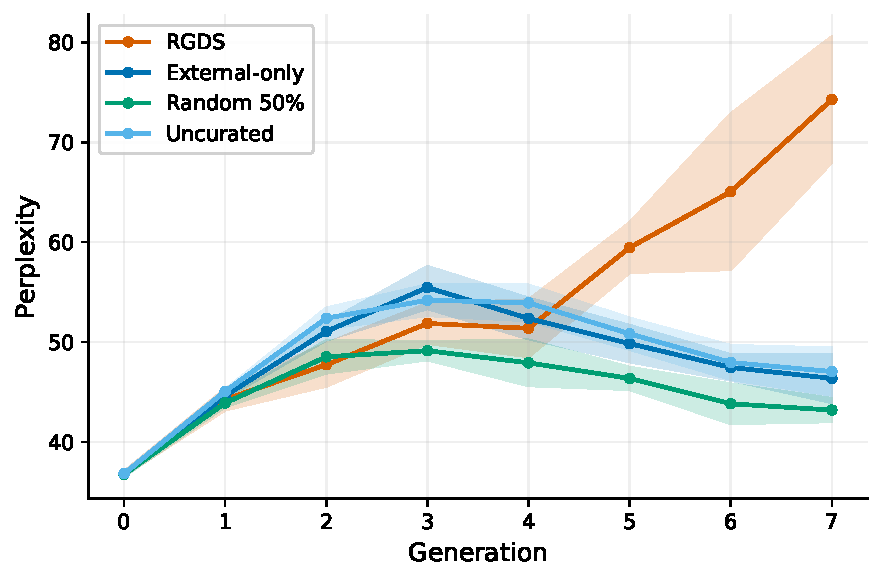
\includegraphics[width=\columnwidth]{figures/fig_ppl_trends.pdf}
\caption{Per-generation perplexity trajectories across four data selection methods (GPT2-125M on WikiText-103). Lines show means over $n{=}3$ seeds; shaded bands show $\pm$1 standard deviation. RGDS diverges from the non-RGDS cluster after Generation~4 and reaches catastrophic perplexity by Generation~7 ($74.29 \pm 7.71$), while the other three methods converge to a narrow band (43--47).}
\label{fig:ppl_trends}
\end{figure}

\begin{figure}[t]
\centering
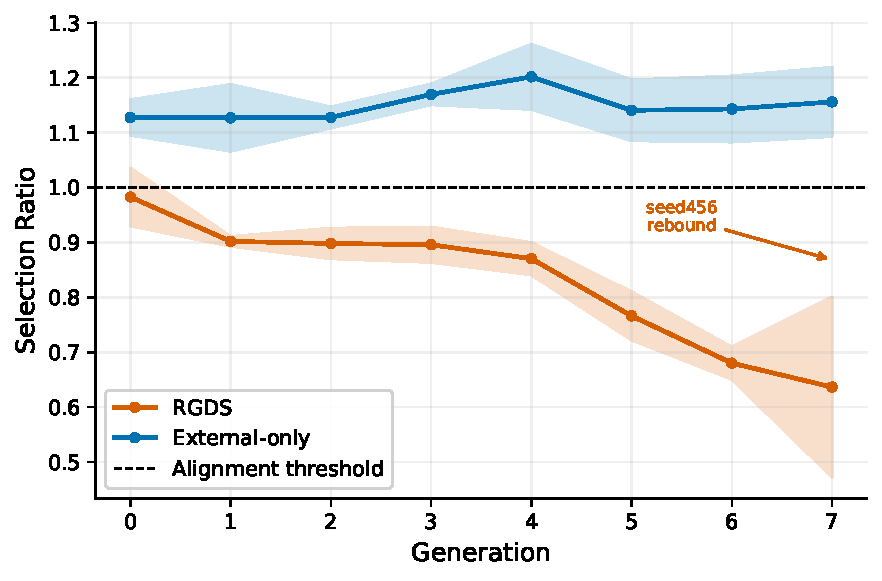
\includegraphics[width=\columnwidth]{figures/fig_ratio_trajectory.pdf}
\caption{Selection ratio trajectories for RGDS and External-only across eight generations. The dashed line marks the alignment threshold ($\text{SR}=1.0$): above it, the selected subset is richer in rare n-grams than the rejected subset; below it, the reverse. RGDS's mean ratio declines from ${\sim}1.0$ to $0.64 \pm 0.20$, while External-only remains above~1.0 throughout. The large variance at Generation~7 reflects seed=456's late rebound (0.65$\to$0.87) without perplexity recovery.}
\label{fig:ratio_trajectory}
\end{figure}

\subsection{RGDS Accelerates Catastrophic Perplexity Degradation}
\label{sec:result_c1}

RGDS is the only method that exhibits catastrophic performance degradation across generations. At Generation~7, RGDS reaches a perplexity of $74.29 \pm 7.71$ ($n{=}3$), compared to $47.04 \pm 2.90$ for Uncurated ($n{=}3$; +58\%) and $43.18 \pm 1.43$ for Random~50\% ($n{=}3$; +72\%). All three seeds show consistent catastrophic degradation---75.07 (seed=42), 81.57 (seed=123), and 66.22 (seed=456)---with all values far exceeding the 43--47 range of the non-RGDS methods. The inter-seed variance of RGDS ($\sigma = 7.71$) substantially exceeds that of any other method ($\sigma \leq 2.97$), reflecting the stochastic dynamics of the co-degradation feedback loop.

The selection ratio traces the mechanism behind this degradation (Figure~\ref{fig:ratio_trajectory}). RGDS's mean selection ratio follows an overall declining trend from ${\sim}1.0$ at Generation~0 to $0.64 \pm 0.20$ at Generation~7 ($n{=}3$). Seeds 42 and 123 reach deeply inverted ratios (0.52 and 0.52 respectively), while seed=456 exhibits a late-generation rebound from 0.65 at Generation~6 to 0.87 at Generation~7---without any corresponding improvement in perplexity (66.22 vs.\ 43--47 for non-RGDS methods). This dissociation between ratio recovery and perplexity indicates that once the embedding space has been sufficiently corrupted, even a partial restoration of selection alignment cannot reverse the accumulated damage to model quality. Across all seeds, the RGDS-selected subset contains fewer rare n-grams than the rejected subset.

\subsection{External Embeddings Avoid the Alignment Gap}
\label{sec:result_c2}

External-only selection applies the identical selection algorithm and 50\% data budget but uses frozen Contriever embeddings. It avoids catastrophic degradation entirely: its Generation~7 perplexity of $46.36 \pm 2.97$ ($n{=}3$) falls within the range of Uncurated ($47.04 \pm 2.90$) and Random~50\% ($43.18 \pm 1.43$).

External-only maintains a selection ratio above~1.0 throughout all generations ($1.16 \pm 0.08$ at Generation~7), indicating continued preferential retention of content-diverse samples.

Since RGDS and External-only differ in exactly one variable---the embedding source---the 27.9-point perplexity gap at Generation~7 ($74.29$ vs.\ $46.36$) is directly attributable to the use of co-degrading internal representations. The selection algorithm is not at fault; the failure is specific to coupling data selection to embeddings that co-evolve with the collapsing model.

Notably, External-only does not significantly outperform Random~50\% in perplexity ($46.36 \pm 2.97$ vs.\ $43.18 \pm 1.43$; $p = 0.198$, Welch's $t$-test, $n{=}3$). Despite maintaining a selection ratio above~1.0, the ``intelligent'' diversity signal from frozen external embeddings provides no measurable advantage over uninformed random subsampling. This null result reinforces the practical implication discussed in \S\ref{sec:discussion}: random sampling is a zero-cost alternative that matches the performance of embedding-guided selection when embeddings are stable and avoids the catastrophic failure when they are not.

\subsection{Internal Selection Underperforms Random Baseline}
\label{sec:result_c3}

The comparison between RGDS and Random~50\% constitutes the cleanest controlled ablation in our design. Both methods operate under identical conditions---same 50\% data budget, same training protocol, same seed infrastructure, same Generation~0 checkpoint---differing only in the selection mechanism: diversity-based curation via the model's own embeddings (RGDS) versus uninformed uniform sampling (Random~50\%). Any performance difference is therefore attributable solely to the selection mechanism, free from the data-volume confound present in comparisons against Uncurated (50\% vs.\ 100\%).

Under this controlled comparison, RGDS exhibits catastrophically worse performance. Its Generation~7 perplexity ($74.29 \pm 7.71$, $n{=}3$) exceeds Random~50\% ($43.18 \pm 1.43$, $n{=}3$) by $+$72\% ($p = .017$, Welch's $t$, $d = 5.61$). The effect is consistent across all three seeds, with each RGDS run (75.07, 81.57, 66.22) far exceeding the non-RGDS cluster ceiling of ${\sim}47$. Internal embedding diversity selection does not merely fail to improve upon random sampling---it actively degrades model quality by a margin that dwarfs all other method differences in this study.

Rare n-gram ratio corroborates the perplexity finding: RGDS retains $0.0061 \pm 0.0009$ at Generation~7, compared to $0.0098 \pm 0.0003$ for Random~50\%---a 38\% reduction in lexical tail content ($p = .014$, $d = -5.66$). The mechanism designed to maximize diversity produces outputs that are measurably \emph{less} diverse than those from uninformed subsampling.

This within-budget contrast should be distinguished from the RGDS vs.\ Uncurated comparison ($+$58\%), which conflates any selection effect with a data quantity difference (50\% vs.\ 100\%). The Random~50\% vs.\ Uncurated comparison (\S\ref{sec:result_s3}) similarly involves a budget confound and does not reach significance ($p = .133$), reinforcing that the within-budget RGDS-vs.-Random ablation provides the most interpretable causal evidence for the alignment gap.

\subsection{Random Pruning: A Directional Observation}
\label{sec:result_s3}

Random~50\% ($43.18 \pm 1.43$, $n{=}3$) achieves lower Generation~7 perplexity than Uncurated ($47.04 \pm 2.90$, $n{=}3$), a reduction of 8.2\% consistent across all three seeds. However, this cross-budget comparison conflates any selection benefit with a data quantity effect (50\% vs.\ 100\%), and the difference does not reach conventional significance ($p = 0.133$, Welch's $t$-test). We report it as a directional observation rather than a confirmed finding, and draw no causal inference about budget effects from this comparison alone.

If confirmed with additional statistical power, this result would suggest that training on a random 50\% subset provides mild regularization compared to using all generated data, consistent with observations that data pruning can improve generalization even without informed selection \citep{sorscher2022beyond}.

While the perplexity difference remains directional, Random~50\% shows a statistically significant advantage in lexical diversity: its Generation~7 rare n-gram ratio ($0.0098 \pm 0.0003$) exceeds Uncurated ($0.0090 \pm 0.0004$) with $p = 0.025$ (two-sided $t$-test, $n{=}3$). Even uninformed subsampling preserves content diversity better than retaining all generated data, suggesting that merely reducing the volume of self-generated training data slows lexical tail erosion.

\subsection{Lexical Diversity Collapse Across Methods}
\label{sec:result_diversity}

RGDS exhibits the sharpest decline in rare token ratio, dropping from approximately 0.010 at Generation~0 to $0.0061 \pm 0.0009$ at Generation~7 (Table~\ref{tab:gen7_summary}). The remaining methods converge to a narrower band: Random~50\% ($0.0098 \pm 0.0003$), Uncurated ($0.0090 \pm 0.0004$), and External-only ($0.0102 \pm 0.0004$). Relative to the WikiText-103 baseline rare token ratio of approximately 0.029, all non-RGDS methods exhibit roughly 65\% lexical tail erosion by Generation~7; RGDS reaches approximately 80\%.

Unlike the perplexity-level normal cluster (ANOVA $p = 0.219$; \S\ref{sec:result_c1}), the rare n-gram differences among non-RGDS methods are statistically significant (ANOVA $p = 0.007$, $n{=}3$ per method). In particular, Uncurated retains significantly fewer rare n-grams than Random~50\% ($p = 0.025$, two-sided $t$-test). Lexical diversity collapse is primarily driven by the iterative self-training loop itself \citep{shumailov2024ai}, but the degree of erosion is modulated by data selection: even uninformed curation (random subsampling) provides measurable protection relative to using all generated data. RGDS is distinctive in accelerating this inherent degradation far beyond all other methods.

\begin{table*}[t]
\centering
\small
\begin{tabular}{llrrrrl}
\toprule
Comparison & Metric & $\Delta$ & Welch $t$ & df & $p$ & Cohen's $d$ \\
\midrule
\multicolumn{7}{l}{\textit{RGDS vs.\ non-RGDS methods}} \\
RGDS vs.\ Random 50\% & PPL & $+$31.10 & 6.88 & 2.1 & .017 & 5.61 \\
RGDS vs.\ External-only & PPL & $+$27.93 & 5.86 & 2.6 & .015 & 4.78 \\
RGDS vs.\ Uncurated & PPL & $+$27.25 & 5.73 & 2.6 & .016 & 4.68 \\
RGDS vs.\ Random 50\% & Rare & $-$.0038 & $-$6.93 & 2.3 & .014 & $-$5.66 \\
RGDS vs.\ External-only & Rare & $-$.0042 & $-$7.51 & 2.6 & .008 & $-$6.13 \\
RGDS vs.\ Uncurated & Rare & $-$.0029 & $-$5.16 & 2.6 & .020 & $-$4.22 \\
\midrule
\multicolumn{7}{l}{\textit{Within-cluster comparisons}} \\
External vs.\ Random 50\% & PPL & $+$3.17 & 1.67 & 2.9 & .198 & 1.36 \\
Random 50\% vs.\ Uncurated & PPL & $-$3.86 & $-$2.07 & 2.9 & .133 & $-$1.69 \\
Random 50\% vs.\ Uncurated & Rare & $+$.0009 & 3.47 & 3.6 & .030 & 2.84 \\
\midrule
\multicolumn{7}{l}{\textit{ANOVA (one-way)}} \\
Non-RGDS (3 methods) & PPL & --- & $F{=}1.98$ & 2,\,6 & .219 & --- \\
Non-RGDS (3 methods) & Rare & --- & $F{=}13.01$ & 2,\,6 & .007 & --- \\
\midrule
\multicolumn{7}{l}{\textit{GPT2-Medium (355M)---$n{=}2$ seeds (42, 123); seed=456 pending}} \\
RGDS vs.\ Random 50\% & PPL & $+$15.15 & \multicolumn{3}{c}{---} & --- \\
RGDS vs.\ External-only & PPL & $+$7.90 & \multicolumn{3}{c}{---} & --- \\
RGDS vs.\ Uncurated & PPL & $-$2.81 & \multicolumn{3}{c}{---} & --- \\
Random 50\% vs.\ Uncurated & PPL & $-$17.96 & \multicolumn{3}{c}{---} & --- \\
\bottomrule
\end{tabular}
\caption{Pairwise statistical comparisons at Generation~7. GPT2-125M rows: $n{=}3$ seeds per method. All pairwise tests use Welch's $t$-test (two-sided, unequal variance). PPL: perplexity on WikiText-103 validation set. Rare: rare trigram ratio. $\Delta$: difference (row method $-$ column method for pairwise; not applicable for ANOVA). Cohen's $d$: standardized effect size. RGDS differs significantly from all non-RGDS methods on both metrics ($p < .05$, $|d| > 4$). Within the non-RGDS cluster, PPL differences are not significant (ANOVA $p = .219$), but rare n-gram differences are (ANOVA $p = .007$). 355M: $n{=}2$ seeds (42, 123); seed=456 pending; $t$-tests deferred until $n \geq 3$.}
\label{tab:stat_tests}
\end{table*}

\subsection{Representation Metrics Do Not Track Content Collapse}
\label{sec:result_rankme}

RankMe values at Generation~7 are comparable across all methods (289--293; Table~\ref{tab:gen7_summary}), with no method showing a meaningfully different value ($292.54 \pm 5.91$ for RGDS vs.\ ${\sim}290$ for non-RGDS methods). The metric designed to track effective embedding dimensionality does not distinguish between catastrophically degraded RGDS and the normally performing alternatives, indicating that embedding structural properties can persist even as the space loses content-discriminative fidelity.

\subsection{Scaling to GPT2-Medium (355M)}
\label{sec:result_scaling}

Results from GPT2-Medium (355M) confirm that model collapse generalizes to larger models and is substantially amplified. Table~\ref{tab:medium_comparison} reports Generation~7 perplexity for all four methods (seed=42 and seed=123 complete for all four methods; all seed=456 experiments pending).%
%TODO(355M-seeds): update when Random seed=123 and all seed=456 complete

\begin{table}[t]
\centering
\small
\begin{tabular}{lcccc}
\toprule
Method & Budget & PPL$_{42}$ & PPL$_{123}$ & $n$ \\
\midrule
Random 50\% & 50\% & 70.25 & 72.55 & 2 \\
External-only & 50\% & 77.74 & 79.56 & 2 \\
RGDS & 50\% & 82.84 & 90.25 & 2 \\
Uncurated & 100\% & 91.66 & 87.05 & 2 \\
\bottomrule
\end{tabular}
\caption{GPT2-Medium (355M) Generation~7 perplexity by seed. PPL$_{42}$ and PPL$_{123}$: WikiText-103 validation perplexity for each seed. RGDS and Uncurated ordering flips across seeds (82.84 vs.\ 91.66 at seed=42; 90.25 vs.\ 87.05 at seed=123). All seed=456 experiments are pending.}
\label{tab:medium_comparison}
\end{table}

\paragraph{C3 holds across scale.} The RGDS two-seed mean (86.55) underperforms Random~50\% (71.40) by +21\% at 355M ($n{=}2$), confirming that internal-embedding diversity selection degrades performance relative to uninformed random sampling regardless of model size. The gap is narrower than at 125M (+72\%, $n{=}3$), but the direction is consistent: co-degrading embeddings produce systematically worse selection than random chance.%
%TODO(355M-seeds): report significance with seed=456

\paragraph{Relative severity shifts at 355M.} At 355M, model collapse is substantially more severe than at 125M across all methods. RGDS and Uncurated converge into a narrow, overlapping band (PPL 83--92) with unstable ordering across seeds: RGDS outperforms Uncurated at seed=42 (82.84 vs.\ 91.66) but underperforms at seed=123 (90.25 vs.\ 87.05). This ordering instability contrasts sharply with the 125M setting, where RGDS consistently exceeded Uncurated by 58\% ($74.29$ vs.\ $47.04$, $n{=}3$). The compression of method differences at high absolute collapse severity is consistent with both the representational redundancy and floor-compression hypotheses discussed in \S\ref{sec:discuss_scaling}. The cross-budget comparison (50\% vs.\ 100\%) remains confounded by data volume differences and should not be interpreted causally. Only the within-budget comparison (RGDS vs.\ Random~50\%, both at 50\%) isolates the effect of the selection mechanism.%
%TODO(355M-seeds): update with seed=456 data

\paragraph{Alignment gap narrows but persists.} The RGDS selection ratio at Generation~7 is $0.85 \pm 0.03$ at 355M ($n{=}2$; 0.83 at seed=42, 0.87 at seed=123), compared to $0.64 \pm 0.20$ at 125M ($n{=}3$). The ratio remains below~1.0---RGDS still preferentially retains content-poor samples---but the inversion is less severe. The +21\% perplexity penalty relative to Random (vs.\ +72\% at 125M) is consistent with this narrower gap.%
%TODO(355M-seeds): confirm ratio trajectory with seed=123 完成后补充完整 4-method 对比和统计检验


\section{Discussion}
\label{sec:discussion}

\subsection{The Embedding Alignment Gap as Goodhart's Law}

The selection ratio trajectory of RGDS---declining from ${\sim}1.0$ at Generation~0 to $0.64 \pm 0.20$ at Generation~7 ($n{=}3$)---instantiates a specific form of Goodhart's law in representation space \citep{gao2023scaling, karwowski2024goodhart}. The proxy measure (embedding diversity) and the true objective (content diversity) are initially correlated: at Generation~0, RGDS's selection ratio exceeds~1, and the method preferentially retains content-rich samples. But as the model trains on its own selected outputs, the embedding space drifts: regions that formerly encoded distinct content merge, effective dimensionality shrinks, and the proxy's correlation with the target degrades.

The selection ratio declining below~1.0 marks the critical transition. Above~1.0, the proxy---while imperfect---points in the right direction. Below~1.0, the proxy has inverted: the model's internal notion of ``diverse'' anti-correlates with content diversity, and selection actively filters out the samples that would slow collapse. With 3-seed data, RGDS's mean ratio begins near~1.0 ($0.98 \pm 0.06$) and falls below~1.0 by Generation~1, never recovering. This degradation is self-reinforcing within the self-training loop because the next generation's embeddings are shaped by the content-depleted training data, further degrading the proxy.

\citet{karwowski2024goodhart} formalize Goodhart's law in the context of reward model overoptimization, showing that proxy performance peaks and then degrades as optimization pressure increases. The embedding alignment gap follows an analogous trajectory: RGDS's mean selection ratio rises slightly in early generations before sustained decline, mirroring the peak-then-degrade pattern characteristic of Goodhart dynamics. The structural difference is that here the proxy (embedding space) is itself a function of the optimization outcome, creating a feedback loop absent from standard Goodhart settings where the proxy is fixed.

The inter-seed variance of the Generation~7 selection ratio ($0.64 \pm 0.20$) reveals an additional nuance. Seeds~42 and~123 reach deeply inverted ratios (${\sim}0.52$), while seed=456 exhibits a late-generation rebound from 0.65 at Generation~6 to 0.87 at Generation~7. Critically, this ratio recovery does not translate into perplexity recovery: seed=456's Generation~7 perplexity (66.22) remains catastrophically elevated relative to the non-RGDS cluster (43--47). This dissociation suggests that the alignment gap operates as a ratchet: once several generations of content-depleted training have degraded model quality, restoring selection alignment at a late stage cannot undo the accumulated distributional damage. The practical implication is that monitoring the selection ratio alone is insufficient---corrective action must be taken \emph{before} the proxy has inverted, not after.

\subsection{The Normal Cluster and the Floor of Self-Training}

Three of our four methods---Random~50\%, External-only, and Uncurated---cluster in a band of Generation~7 perplexities between 43 and 51 despite substantial differences in design (ANOVA $p = 0.219$, $n{=}3$ per method). Random selection applies no intelligent curation; External-only applies greedy diversity maximization with frozen embeddings; Uncurated retains all data without filtering. That these methods converge to comparable PPL outcomes indicates that the floor of perplexity degradation in this self-training protocol is determined by the iterative feedback loop itself \citep{shumailov2024ai}, not by the data selection strategy.

Critically, this convergence is specific to perplexity. When measured by rare n-gram ratio, the same three methods show statistically significant differences (ANOVA $p = 0.007$): Uncurated retains fewer rare n-grams ($0.0090 \pm 0.0004$) than both Random~50\% ($0.0098 \pm 0.0003$) and External-only ($0.0102 \pm 0.0004$). Content diversity can degrade silently---without perplexity penalty---indicating that PPL alone is insufficient to capture all dimensions of model collapse.

This convergence is consistent with theoretical analyses showing that self-consuming generative processes converge toward the modes of the original distribution regardless of training procedure \citep{seddik2024how}. Within the non-catastrophic regime, data selection method variation produces second-order effects relative to the first-order dynamics of iterative self-training. RGDS is the outlier precisely because it introduces a systematic bias---toward content-depleted samples---that compounds across generations, pushing it outside the natural convergence band.

\subsection{Why the Alignment Gap Narrows with Scale}
\label{sec:discuss_scaling}

The within-budget comparison (RGDS vs.\ Random~50\%, both at 50\%) reveals that scaling reduces the alignment gap penalty: the absolute PPL gap contracts from 31.10 at 125M ($n{=}3$) to 15.15 at 355M ($n{=}2$), and the relative gap narrows from $+$72\% to $+$21\%.%
%TODO(355M-seeds): confirm with 3-seed data
Two mechanisms---not mutually exclusive---may underlie this attenuation.

\emph{Representational redundancy.} Larger models begin self-training with higher effective embedding dimensionality: GPT2-Medium's Generation~0 RankMe (${\sim}365$) exceeds GPT2-125M's (${\sim}276$) by 33\%. This additional representational capacity buffers the geometric distortion that drives proxy inversion \citep{jing2022understanding}---more dimensions carry meaningful signal, so the eigenvalue-based selection objective tracks genuine content distinctions for longer. Consistent with this mechanism, the RGDS selection ratio at Generation~7 improves from $0.64 \pm 0.20$ (125M, $n{=}3$) to $0.85 \pm 0.03$ (355M, $n{=}2$), indicating that proxy-target alignment degrades more slowly at larger scale.

\emph{Compression under severe collapse.} The 355M Uncurated baseline degrades far more severely than at 125M (PPL~$89.36$, $n{=}2$, vs.\ $47.04 \pm 2.90$, $n{=}3$). When absolute collapse is severe, method differences may compress toward a common degradation trajectory, shrinking the relative gap between RGDS and Random~50\% independently of representational improvement. The absolute gap contracts from 31.10 to 15.15, consistent with---but not diagnostic of---either explanation.

Moreover, the gap compression is specific to RGDS. External-only's penalty relative to Random~50\% increases from $+$7.4\% at 125M ($n{=}3$) to $+$10.2\% at 355M ($n{=}2$), and Uncurated's penalty increases from $+$8.9\% to $+$25.1\%.%
%TODO(355M-seeds): confirm with 3-seed data
A uniform compression effect would shrink all method differences symmetrically; the observed asymmetry---where only the alignment-gap-driven penalty contracts while other penalties widen---is directionally consistent with representational redundancy as a contributing factor.

These two effects likely co-exist, and the observed attenuation reflects their joint action. The absolute penalty persists---RGDS remains 21\% worse than Random~50\% at 355M ($n{=}2$)---but the alignment gap is attenuated, not eliminated. Definitively distinguishing between representational redundancy and floor-compression effects requires experiments at three or more model scales. The asymmetric gap pattern at 355M---where only the alignment-gap-driven penalty contracts while other method differences expand---provides directional evidence consistent with representational redundancy, but does not rule out scale-dependent floor compression.%
%TODO(355M-seeds): confirm with seed=456 data

\subsection{Practical Implications}

The results yield a direct prescription: do not use the training model's own embeddings for data selection in iterative self-training settings. Any embedding-based curation method whose embedding source co-evolves with the model---including methods based on facility location objectives, kernel density estimation, or clustering over internal representations---is vulnerable to the same proxy-target inversion. The risk is highest when curation occurs at every generation and no external anchor stabilizes the embedding space.

Random sampling provides a zero-cost alternative that avoids the alignment gap entirely and, in our experiments, slightly outperforms both Uncurated and External-only baselines (though the difference is not statistically significant at $n{=}3$; \S\ref{sec:result_s3}). When informed selection is desired, frozen external embeddings maintain selection quality across generations at the cost of an additional inference pass through the external encoder.

\subsection{Connection to Concept Drift}

The embedding alignment gap can be understood as a special case of concept drift \citep{lu2019learning, gama2014survey} in which the drift is endogenous: the model's own outputs define its future training distribution, which in turn reshapes its representations. In standard concept drift settings, the data distribution shifts due to external factors, and the model must adapt. In self-consuming training, the model \emph{causes} the distribution shift, creating a feedback loop where representation degradation and distributional shift co-amplify.

This endogenous drift is particularly insidious for embedding-based data selection because the selection mechanism relies on the very representations undergoing drift. Concept drift detection methods that monitor distributional divergence between training batches would flag the symptom (changing distributions) but not the cause (embedding-selection feedback). Addressing this failure mode requires either anchoring selection to a stable external reference---as External-only does---or monitoring the selection ratio to detect proxy inversion before it compounds.

\subsection{Limitations}

Several limitations scope our conclusions:
\begin{enumerate}
    \item Our experiments use GPT2-125M ($n{=}3$) and GPT2-Medium (355M, $n{=}2$); the embedding alignment gap may manifest differently in larger models with richer representational capacity.
    \item We train and evaluate exclusively on WikiText-103; other domains (code, dialogue, scientific text) may exhibit different collapse dynamics.
    \item Our self-training protocol uses cumulative fine-tuning with fixed hyperparameters; instruction-tuning and RLHF pipelines introduce additional variables (reward signals, preference data) that could interact with the alignment gap.
    \item Our analysis of dimensional collapse is empirical and analogical \citep{jing2022understanding}---we do not provide a formal theoretical proof linking effective dimensionality reduction to selection ratio decline.
    \item GPT2-Medium results are based on two seeds ($n{=}2$); full three-seed confirmation is pending.
    \item We fix the selection budget at 50\%. Lower budgets (e.g., 30\%) would amplify any selection bias---including the alignment gap---by concentrating training on a smaller, more aggressively filtered subset. Higher budgets (e.g., 70\%) would dilute the selection signal and approach the Uncurated baseline. Our 50\% budget represents a moderate operating point; the alignment gap's sensitivity to budget fraction is an open question.
    \item We extract embeddings from the last hidden layer. Intermediate layers or pooled representations may exhibit different alignment dynamics; exploring this design choice is left to future work.
\end{enumerate}

\subsection{Future Work}

Three directions extend this work. First, scaling to 1B+ parameter models would test whether richer embedding spaces resist or amplify the alignment gap. Second, replicating across diverse pretraining corpora (OpenWebText, C4, The Pile) would establish domain generality. Third, \emph{embedding re-anchoring} strategies---periodically resetting the selection embeddings to an external encoder or a cached earlier checkpoint---could retain the benefits of informed selection while preventing proxy inversion. Finally, a theoretical analysis relating the selection ratio trajectory to the rate of effective dimensionality reduction would provide a predictive framework for identifying when the alignment gap becomes critical before the proxy has fully inverted.


\section{Conclusion}
\label{sec:conclusion}

This work introduces the \emph{embedding alignment gap}---the progressive decorrelation between a model's internal embedding similarity and actual content diversity during iterative self-training---and demonstrates its consequences for embedding-based data curation. Through controlled self-training experiments with GPT2-125M over eight generations, we establish three principal findings.

First, the embedding alignment gap is real and self-reinforcing. The internal embedding diversity selection ratio begins near the alignment threshold (${\sim}1.0$) at Generation~0 and declines progressively to $0.64 \pm 0.20$ by Generation~7 ($n{=}3$), indicating that the model's own embeddings increasingly select \emph{against} content-rich samples. As the ratio falls below~1.0---which occurs in all three seeds by Generation~1---the proxy inverts: diversity-maximizing selection over internal embeddings actively accelerates the loss of content diversity.

Second, this proxy inversion has catastrophic practical consequences. Representation-guided diversity selection (RGDS) using internal embeddings produces Generation~7 perplexity over 70\% higher than random baseline at the same 50\% data budget ($74.29 \pm 7.71$ vs.\ $43.18 \pm 1.43$, $n{=}3$). Meanwhile, Random~50\% ($43.18 \pm 1.43$), External-only ($46.36 \pm 2.97$), and Uncurated ($47.04 \pm 2.90$) converge to a statistically indistinguishable cluster ($n{=}3$), confirming that the catastrophic degradation of RGDS is not an artifact of data reduction but a direct consequence of co-degrading embeddings.

Third, standard representation quality diagnostics fail to detect the alignment gap. Both RankMe effective dimensionality and $k$-NN probing accuracy remain stable throughout the collapse trajectory, rendering the proxy inversion invisible to conventional monitoring tools.

These findings carry several caveats. Our experiments are limited to GPT2-scale models, a single pretraining corpus, and a fixed self-training protocol; the generality of these results to larger models, diverse domains, and alternative training paradigms remains to be established (see the limitations and future directions discussed in \S\ref{sec:discussion}).

The practical implication is direct: internal embeddings that co-evolve with the training model should not serve as the selection criterion in iterative self-training pipelines. Random sampling---requiring no additional computation---provides a robust alternative that avoids proxy inversion entirely. When informed selection is desired, frozen external embeddings maintain alignment across generations. For practitioners who cannot abandon internal embeddings, the selection ratio offers a lightweight, real-time diagnostic: an overall declining trend below~1.0 signals that selection has begun to work against its intended objective, and corrective action---such as re-anchoring to an external encoder---should be taken before the degradation compounds.


\bibliography{references}

\end{document}
